Die offizielle Definition des Modbus Protokolls von der Modbus Organization \cite{Modbus_Organization_AP:2012} lautet:
\begin{quotation}
	\emph{
		MODBUS is an application layer messaging protocol, positioned at level 7 of the OSI model, which provides client/server communication between devices connected on different types of buses or networks.}
\end{quotation}

Der Modbus Standard definiert ein Application Layer Kommunikations Protokoll, dass sich auf Schicht 7 des OSI-Modells befindet. Es bietet Client/Server Kommunikation zwischen Geräten, die auf verschiedenen Bussen oder Netzwerken angeschlossen sind.

Das Modbus Protokoll wurde 1979 von der Firma Gould-Modicon entwickelt. Besonders wird das Protokoll in Mess- und Regelsystemen eingesetzt, da es speziell für die Kommunikation mit speicherprogrammierbaren Steuerungen entwickelt wurde. Das Modbus Protokoll ist ein Industriestandard. Es bietet einen universellen Übertragungsweg, ganz egal welches Übertragungsmedium genutzt wird. Es funktioniert sowohl über ein serielles Bussystem, als auch über eine Netzwerkverbindung. Außerdem können mit sogenannten Protokollumsetzern Geräte mit serieller Kommunikation in ein Netzwerksystem eingebettet werden. Durch den Einsatz von Paritätsprüfungen und Checksummen gewährleistet das Protokoll eine zuverlässige Übertragung. \cite{KUNBUS_GmbH:o.J., kvm-concepts_GmbH:2022}


Die folgende theoretische Beschäftigung mit dem Modbus Protokoll bezieht sich wenn nicht anders angegeben auf die offiziellen Modbus Dokumentationen \cite{Modbus_Organization_AP:2012, Modbus_Organization_SL:2012}. 

Da das Modbus Protokoll nur Layer 7 definiert, kann es in verschiedenen Übertragungssystemen implementiert werden:
\begin{itemize}
	\item \textbf{Modbus TCP/IP:} Die Geräte sind an einem Netzwerk angeschlossen und kommunizieren via TCP/IP.
	\item \textbf{Modbus Serial Line:} Die Geräte sind hier an einem seriellen Bus angeschlossen. Dabei gibt es zwei Übertragungsarten, nämlich RTU und ASCII. Genauere Beschreibungen der beiden Übertragungsarten finden sich später in diesem Kapitel.
	\item \textbf{Modbus Plus:} Funktioniert mittels eines Tokens. Jeweils das Gerät, welches den Token aktuell besitzt, ist der Client und kann die Kommunikation mit den anderen Geräten initialisieren. Wenn der derzeitige Client keine Nachrichten mehr senden muss, gibt er den Token an das nächste Gerät weiter \cite{Rinaldi:2016}.
\end{itemize}

Folgende Grafik (\ref{fig:modbus_stack}) illustriert horizontal die unterschiedlichen Übertragungssysteme und vertikal welche Schichten von darunterliegenden Protokollen und Technologien besetzt werden.
\begin{figure}[H]
	\centering
	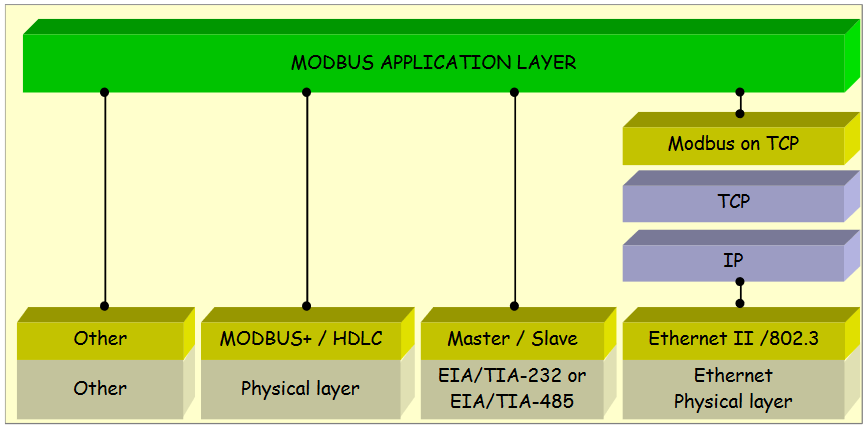
\includegraphics[width=1.0\linewidth]{Bilder/Modbus_layers}
	\caption{Modbus Stack (Quelle: \url{https://modbus.org/docs/Modbus_Application_Protocol_V1_1b3.pdf})}
	\label{fig:modbus_stack}
\end{figure}

\subsection{Funktionsweise} \label{modbus_funktionsweise}
Modbus verwendet das Client/Server System. In einem Bussystem kann es nur einen Client geben. Es können jedoch beliebig viele Server am Bus angeschlossen werden. Der Client kann die Kommunikation mit den einzelnen Servern initialisieren. Er kann ihnen Daten senden und von ihnen Daten anfordern. Ein Server hingegen kann keine Kommunikation beginnen, sondern lediglich auf Anfrage des Clients handeln.

Jeder Server am Bus hat eine einzigartige Adresse. Die Adressen können Werte von 0 bis 255 einnehmen (siehe Tab.~\ref{tab:modbus_adressen} für die Einteilung). 
\begin{table}[h]
	\caption{Modbus Adressen Einteilung \label{tab:modbus_adressen}}
	\begin{tabularx}{\textwidth}{@{}c|c|X@{}}
		\toprule
		\textbf{Adressen} & \textbf{Bezeichnung} & \textbf{Beschreibung} \\
		\midrule
		0 & Broadcast & Hiermit sendet der Client eine Anfrage an alle Server am Bus. Diese senden keine Antwort zurück. \\
		1 - 247 & Server & Der Client kann damit einzelne Server ansprechen. Diese senden dem Client eine Antwort zurück. \\
		248 - 255 & Reserviert & \\
		\bottomrule
	\end{tabularx}
\end{table}

Der Grundbestandteil des Modbus Protokolls ist die sogenannte \acf{pdu}. Diese besteht aus dem Function Code und den Daten. Sie sind für den Empfänger relevant. Damit die Übertragung zwischen Client und Server funktionieren kann, werden dem \acs{pdu} zusätzliche Felder hinzugefügt. Es wird die Adresse des angefragten Servers und eine Checksumme zur Fehlererkennung eingebaut. Das gesamte Datenpaket wird \acf{adu} genannt.
(siehe Abb.~\ref{fig:modbus_adu_pdu}).
\begin{figure}[ht]
	\centering
	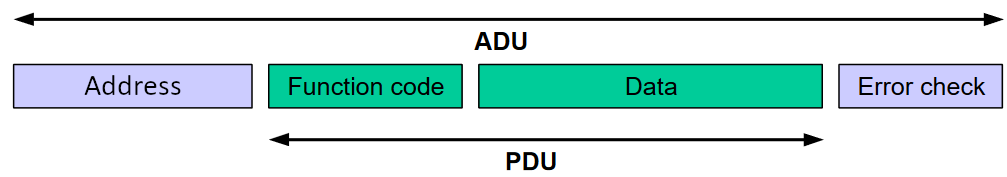
\includegraphics[width=1.0\linewidth]{Bilder/General_Modbus_Frame_Changed}
	\caption{Modbus Dataframe (Quelle: \url{https://modbus.org/docs/Modbus_Application_Protocol_V1_1b3.pdf} [angepasst])}
	\label{fig:modbus_adu_pdu}
\end{figure}

\begin{itemize}
	\item \textbf{Address Field:} Die Adresse des angefragten Servers bzw. mehrerer Server.
	\item \textbf{Function Code:} Dieses Feld ist ein Byte groß. Die Werte reichen von 1 bis 255, wobei 128 bis 255 für Fehlercodes vorbehalten sind. Wenn der Server eine Nachricht vom Client bekommt, zeigt ihm dieses Feld den Verwendungszweck der erhaltenen Daten an. 
	\item \textbf{Data:} In diesem Feld werden die Daten beigefügt. Außerdem sind zusätzliche Informationen wie die Registeradressen und die Länge der Daten enthalten. Teilweise kann dieses Feld auch Leer bleiben. In diesem Fall werden alle nötigen Informationen über die auszuführende Aktion durch den Function Code geliefert.
	\item \textbf{Error Check:} Falls bei der Übertragung einzelne Bits verändert oder verloren gehen, kann mit der Checksumme die Vollständigkeit der erhaltenen Nachricht festgestellt werden. Der Client bildet aus der zu versendenden Nachricht eine Checksumme und hängt sie der Nachricht an. Der Server erhält die Nachricht und bildet ebenfalls eine Checksumme aus der erhaltenen Nachricht. Nun vergleicht der Server die errechnete mit der erhaltenen Checksumme und determiniert, ob diese ident (kein Fehler) oder unterschiedlich (Übertragungsfehler) sind. Bei einem Fehler sendet er einen entsprechenden Fehlerfunktionscode zurück.
\end{itemize}

Die Datenspeicherung von Modbus basiert auf sogenannten Registern. Die Register werden im Speicher des jeweiligen Geräts in einem Block zusammengefasst. Es gibt verschiedene Registertypen, die sich in der Länge der gespeicherten Daten und dem Zugriffstyp unterscheiden (siehe Tab.~\ref{tab:modbus_register}). \newline Ein Client kann die Register auf einem Server mittels Anfragen auslesen oder setzen. Server können ihre eigenen Register setzen.
\begin{table}[H]
	\caption{Modbus Registertypen \label{tab:modbus_register}}
	\begin{tabularx}{\textwidth}{@{}l|c|c|X@{}}
		\toprule
		\textbf{Registertyp} & \textbf{Datentyp} & \textbf{Zugriffstyp} & \textbf{Beschreibung} \\
		\midrule
		Input Discrete & Single bit & Read-Only & Durch \acf{io} veränderbar \\
		Coils & Single bit & Read-Write & Durch Anfragen veränderbar \\
		Input Registers & 16-bit word & Read-Only & Durch \acs{io} veränderbar \\
		Holding Registers & 16-bit word & Read-Write & Durch Anfragen veränderbar \\
		\bottomrule
	\end{tabularx}
\end{table} 
\cite{IPC2U_GmbH:o.J.}

Jeder dieser Blöcke hat einen separaten Bereich im Speicher (Siehe Abb.~\ref{fig:modbus_register_many_blocks}):
\begin{figure}[H]
	\centering
	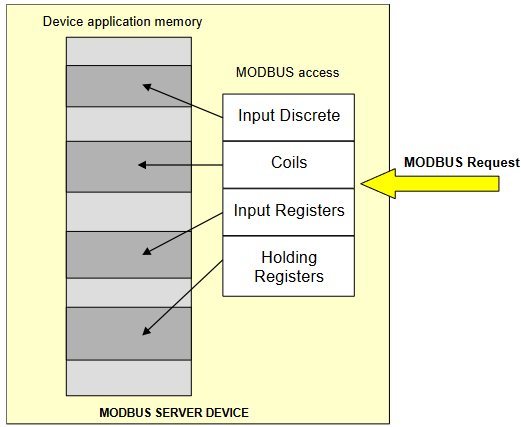
\includegraphics[width=0.4\linewidth]{Bilder/Modbus_Data_Model_with_separate_block}
	\caption{Modbus Daten in separaten Blöcken (Quelle: \url{https://modbus.org/docs/Modbus_Application_Protocol_V1_1b3.pdf})}
	\label{fig:modbus_register_many_blocks}
\end{figure}

Oder die Blöcke sind zusammengeschaltet und können durch unterschiedliche Eingaben erreicht werden (Abb.~\ref{fig:modbus_register_one_block}).
\begin{figure}[H]
	\centering
	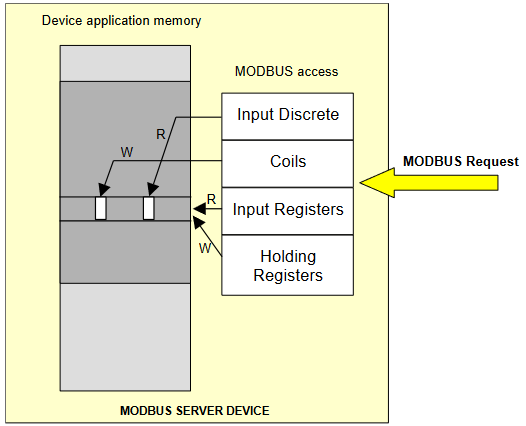
\includegraphics[width=0.4\linewidth]{Bilder/Modbus_Data_Model_with_one_block}
	\caption{Modbus Daten in einem Block (Quelle: \url{https://modbus.org/docs/Modbus_Application_Protocol_V1_1b3.pdf})}
	\label{fig:modbus_register_one_block}
\end{figure}

\subsection{Übertragungsarten} \label{modbus_uebertragungsarten}
Es gibt verschiedene Übertragungsarten. Für die serielle Schnittstelle, gibt es \acf{rtu} und \acf{ascii}. Auf einem seriellen Bus, müssen alle Geräte die selbe Übertragungsart verwenden. Der \acs{rtu} Modus ist dabei der Standard, den alle Modbus Geräte implementieren müssen. \acs{ascii} kann optional verwendet werden. \newline Es gibt auch noch \acs{tcp} und Modbus Plus. Diese beiden Übertragungsarten sind für diese Diplomarbeit nicht relevant. Daher wird auf eine genauere Beschreibung verzichtet.

\paragraph{\acs{rtu} Modus}
Bei dem \acs{rtu} Modus werden 8-bit Datenbytes nacheinander gesendet. In den meisten Programmen werden diese 8-Datenbits von 2 hexadezimalen Zahlen dargestellt. Die Übertragung muss dabei ununterbrochen stattfinden. Im Vergleich zu \acs{ascii} ist bei \acs{rtu} der Datendurchsatz höher. 

Zusätzlich zu den 8 Datenbits kommen noch 3 Hilfsbits dazu. Für jedes übertragene Datenbyte, werden somit 11 Bits verschickt. Diese werden folgendermaßen aufgeteilt:
\begin{itemize}
	\item \textbf{1 Startbit:} Signalisiert dem Empfänger, dass die Übertragung anfängt
	\item \textbf{8 Datenbits:} Die eigentlichen Daten
	\item \textbf{1 Paritätsbit:} Stellt fest, ob alle Datenbits richtig empfangen wurden. Es zeigt an, ob die Summe der empfangene Datenbits gerade (even) oder ungerade (odd) ist. Ob die Summe gerade ist oder ungerade wird dann mit dem Paritätsbit verglichen \cite{IBM_Corporation:2023} (vlt. noch genauer beschreiben; wie das verglichen wird). Es können 3 verschiedene Modi eingestellt werden: even, odd oder no parity. 
	\item \textbf{1/2 Stopbits:} Signalisiert dem Empfänger, dass die Übertragung endet. Falls no parity eingestellt wurde, gibt es 2 Stopbits, dafür aber kein Paritätsbit.
\end{itemize}

Nach jeder Nachricht wird 3,5 Zeichen gewartet, bis die nächste Nachricht versendet wird. Dadurch erkennt das Protokoll genau, ob ein empfangenes Datenbyte noch zur vorherigen Nachricht gehört oder ob bereits die nächste Nachricht anfängt.
Der Aufbau eines Modbus RTU Frames ist in Abb.~\ref{fig:modbus_frame} zu sehen.
\begin{figure}[H]
	\centering
	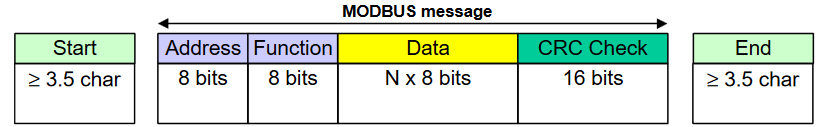
\includegraphics[width=1.0\linewidth]{Bilder/Modbus_frame}
	\caption{Modbus RTU Frame (Quelle: \url{https://www.modbus.org/docs/Modbus_over_serial_line_V1.pdf})}
	\label{fig:modbus_frame}
\end{figure}

Zur Berechnung der Checksumme wird die \acf{crc} Methode verwendet. Diese wird auf den gesamten Inhalt der Nachricht (\acs{adu}) angewandt. Es wird ein 16 Bit Wert generiert, der der Nachricht angehängt wird. Berechnet wird das, indem jeweils die 16 Bit im \acs{crc} Feld mit je 8 Bit der Nachricht XOR verknüpft werden. Nach jeder XOR Verknüpfung werden die Bits 8 mal verschoben und jedes mal mit einem fixierten Wert XOR verknüpft. 

Diese Übertragungsart wird in den Geräten bei Bösch verwendet. Daher verwendet auch die RLT Anzeige den \acs{rtu} Modus.

\paragraph{\acs{ascii} Modus}
Im \acs{ascii} Modus werden \acs{ascii} Zeichen verschickt. Anders als beim \acs{rtu} Modus bedarf es keiner Pause zwischen zwei Nachrichten. Eine neue Nachricht wird mit dem ":" Zeichen eingeleitet und mit "CR" und "LF" (im Glossar: carriage return + line feed) beendet.

Anders als beim \acs{rtu} Modus werden nur 7 Datenbits versendet. \acs{ascii} benötigt ebenfalls 3 Hilfsbits. Deswegen auch der geringere Datendurchsatz, da bei \acs{rtu} 3 Hilfsbits auf 8 Datenbits treffen. Diese insgesamt 10 Bits werden folgendermaßen aufgeteilt:
\begin{itemize}
	\item \textbf{1 Startbit}
	\item \textbf{7 Datenbits}
	\item \textbf{1 Paritätsbit}
	\item \textbf{1/2 Stopbits}
\end{itemize}

Zur Berechnung der Checksumme wird die \acf{lrc} Methode verwendet. Diese wird auf den Inhalt der Nachricht angewandt, Start- und Endzeichen sind ausgenommen. Es wird ein 8 Bit Wert generiert, der der Nachricht angehängt wird. Berechnet wird das, indem jeweils 8 Bit der Nachricht addiert werden. Die Überträge werden vernachlässigt.

\subsection{Serielle Kommunikation über RS485}
Serielle Kommunikation bedeutet grundsätzlich, dass eine Nachricht Bit für Bit (seriell) versendet wird \cite{Schnabel:o.J.}. Dafür gibt es verschiedene Standards, die unterschiedliche Kriterien aufweisen (siehe Tabelle \ref{tab:serielle}) 
\begin{table}[H]
	\caption{Serielle Kommunikation Standards \label{tab:serielle}}
	\begin{tabularx}{\textwidth}{@{}X|c|c|c@{}}
		\toprule
		\textbf{Anschlussname} & \textbf{RS232} & \textbf{RS422} & \textbf{RS485}\\
		\midrule
		Übertragungsart & Vollduplex & Vollduplex & Halb- oder Vollduplex \\
		Maximale Distanz & 15 Meter & 1200 Meter & 1200 Meter \\
		Topologie & Point-to-Point & Point-to-Point & Multi-point \\
		\bottomrule
	\end{tabularx}
\end{table}
\cite{IPC2U_GmbH_SerielleSchnittstellen:o.J.}

In den Lüftungsgeräten der Firma Bösch wird die RS485 Schnittstelle verwendet.

\paragraph{RS485} \label{rs485}
RS485 ist ein Standard, welcher die elektrischen bzw. physikalischen Eigenschaften einer Schnittstelle definiert. Es befindet sich auf Schicht 1 des ISO/OSI Modells. Der Standard definiert nicht die Struktur der zu übertragenen Daten. Daher kann es in Kombination mit den unterschiedlichsten Protokollen, auf den darüber liegenden Schichten verwendet werden (z.B. Modbus RTU) \cite{Janitza:o.J.}.

RS485 verwendet für das Übertragen 2 Leitungen. Es gibt eine Leitung, auf der das Datenbit übertragen wird. Wenn das Datenbit 1 ist, ist ein High Spannungspegel auf dieser Leitung, wenn das Datenbit 0 ein Low Spannungspegel. Auf der zweiten Leitung wird das invertierte Datenbit übertragen. Wenn das Datenbit 1 ist, ist ein Low Spannungspegel auf dieser Leitung, wenn das Datenbit 0 ein High Spannungspegel. Der Spannungsunterschied zwischen den beiden Leitungen muss beim Übertragen mindestens 1,5V betragen \cite{Kugelstadt:2021}. 
Eine Darstellung der Spannungspegel der beiden Leitungen (dargestellt in Rot und Blau) beim Übertragen findet sich in Abb.~\ref{fig:rs485_signal}.
\begin{figure}[H]
	\centering
	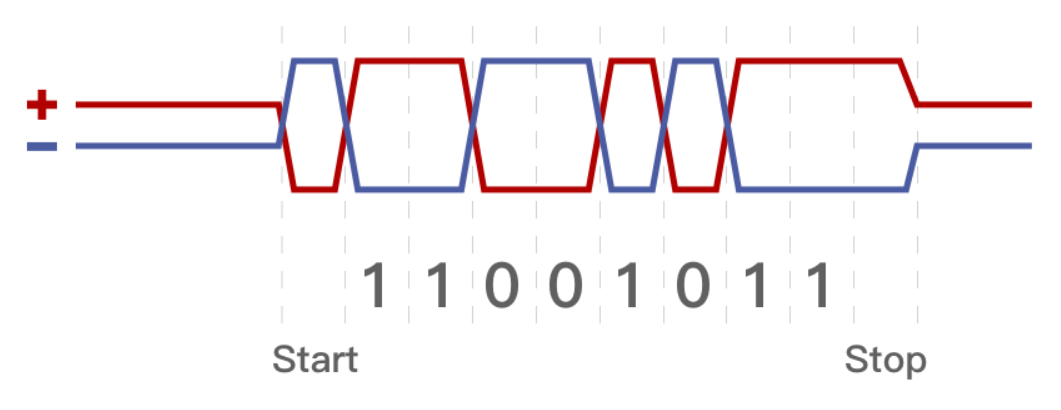
\includegraphics[width=0.5\linewidth]{Bilder/RS485_signal_illustration}
	\caption{RS485 Signal (Quelle: \url{https://www.lorric.com/en/WhyLORRIC/Flowmeter/what-is-rs485})}
	\label{fig:rs485_signal}
\end{figure}

Dadurch, dass es 2 Leitungen gibt und die Spannungsunterschiede genügend groß definiert sind, ist RS485 ziemlich Resistent gegen elektromagnetische Störungen. Die Daten können auch über längere Strecken sicher übertragen werden. \cite{Kugelstadt:2021, Heinen_Elektronik_GmbH:o.J.}. \\

RS485 kann entweder im Halb- oder Vollduplex Modus aufgesetzt werden. \newline Halbduplex bedeutet, dass entweder gesendet oder empfangen werden kann, aber nicht beides gleichzeitig. Der Bus benötigt nur 1 Leitungspaar (2 Leitungen). \newline Vollduplex bedeutet, dass Senden und Empfangen parallel funktioniert. D.h. es gibt 2 Leitungspaare (4 Leitungen), eine für das Senden, eine für das Empfangen \cite{Kugelstadt:2021}. \\

Eine wichtige Information, die uns durch unseren Firmenbetreuer mitgeteilt wurde, ist, dass der Bus nach dem letzten Teilnehmer einen Terminierungswiderstand benötigt. Dadurch lässt sich eine Reflexion des Signals verhindern. (vgl. \cite{Kugelstadt:2021}). Auf den QBM Geräten gibt es dafür einen Schalter, mit diesem man den Terminierungswiderstand ein bzw. ausschalten kann. Da die Existenz dieses Schalters während der praktischen Ausarbeitung unserer Diplomarbeit lange vergessen wurde, kam es beim Testen diverse male zu scheinbar unerklärlichen Fehlern.

\paragraph{Baudrate} \label{baud_rate}
Die Baudrate stellt die Schrittgeschwindigkeit in einem seriellen Bussystem dar. Die Baudrate wird häufig mit der Maßeinheit Bit/s verwechselt. Obwohl beide den Datendurchsatz darstellen, misst die Baudrate wie viel Zeit für einen Schritt benötigt wird und nicht wie viele Bits pro Sekunde übertragen werden. Diese beiden Werte können, müssen aber nicht immer gleich sein. Ein Schritt ist dabei definiert als eine Änderung des Signals. 
\cite{KUNBUS_GmbH_Baudrate:o.J.}
In dieser Diplomarbeit wird dennoch der Begriff Baudrate verwendet, obwohl die in den Konfigurationsdateien angegebenen Datenraten in Bit/s gemessen werden. Die Bezeichnung Baudrate wurde deswegen gewählt, da sie in der Industrie weit verbreitet ist. Gängige Baudraten sind für Modbus 9600 Bit/s und 19200 Bit/s.
